   
\documentclass[11pt]{article}
\usepackage{amsmath,amsthm,verbatim,amssymb,amsfonts,amscd, graphicx}
\usepackage{graphicx}
\usepackage{listings}
\usepackage{float}
\usepackage{url}
\usepackage{titlesec}
\setcounter{secnumdepth}{4}




\graphicspath{{./times/}}
\topmargin0.0cm
\headheight0.0cm
\headsep0.0cm
\oddsidemargin0.0cm
\textheight23.0cm
\textwidth16.5cm
\footskip1.0cm

\titleformat{\paragraph}
{\normalfont\normalsize\bfseries}{\theparagraph}{1em}{}
\titlespacing*{\paragraph}
{0pt}{3.25ex plus 1ex minus .2ex}{1.5ex plus .2ex}


\begin{document}
\title{CS 5220\\ Project 3 - Floyd-Warshall Algorithm}
\author{Eric Gao (emg222)\\ Elliot Cartee (evc34)\\ Sheroze Sheriffdeen(mss385)}
\maketitle

\section{Introduction}
The Floyd-Warshall algorithm computes the pair-wise shortest path lengths given a graph with a metric. The computational pattern of this algorithm is very much akin to matrix multiplication. If $l_{ij}^s$ represents the the length of the shortest path from node $i$ to $j$ in at most $2^s$ steps, \cite{writeup} then
\begin{equation}
	l_{ij}^{s+1} = \min_k \{ l_{ik}^s + l_{kj}^s \}
\end{equation} 

\section{Design Decisions}
 
\subsection{Parallel Tuning}
\subsection{MPI}

In the MPI implementation, each process handles a certain region of the graph. To prevent a master process orchestrating the distance computation, we ideally want each process to only wait for information from the relevant part of the graph. To that end, we take the adjacency matrix on which the Floyd-Warshall algorithm is run and partition the graph by chunks of columns. 

\begin{figure}[H]
\centering
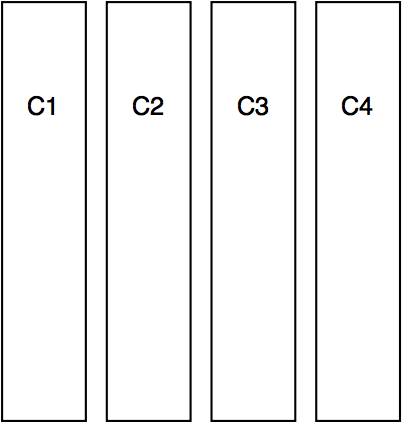
\includegraphics[scale=0.2]{initial_partition.png}
\caption{Initial partition of the graph where each $C_i$ is a sequence of columns}
\label{fig:init_part}
\end{figure}

Now each sequence of columns owned by a processor can be decomposed into square blocks. To compute the next iteration of the Floyd-Warshall algorithm for a single block, say block number $i$ in processor $2$, we need the $i^{th}$ block from all other processors.

\begin{figure}[H]
\centering
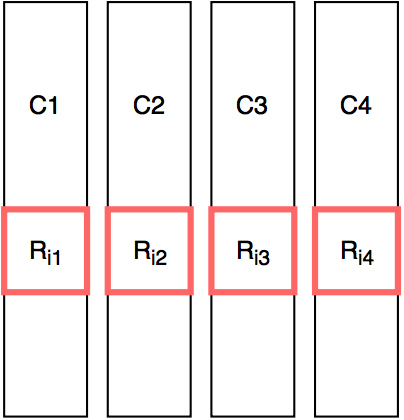
\includegraphics[scale=0.2]{allgather.png}
\caption{For block $R_{i1}$ we need the $i^{th}$ block from all other processors}
\label{fig:allgather}
\end{figure}

Therefore, we do an \texttt{MPI\_Allgather} operation which gathers the $i^{th}$ block from all the processors and recreates the $i^{th}$ row chunk in all processors. Now, we can update block $R_{ij}$ for all $j$ processors. 

\begin{figure}[H]
\centering
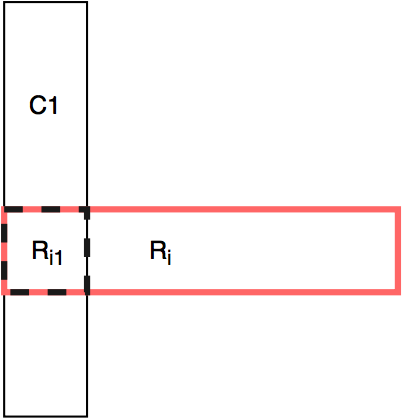
\includegraphics[scale=0.2]{row_col.png}
\caption{Updating the $i^{th}$ square block by processor 1 using row chunk $i$}
\label{fig:row_col}
\end{figure}

The \texttt{MPI\_Allgather} is then repeated until all square blocks have completed a step in the Floyd-Warshall algorithm. Each processor individually checks whether an update was made to their sequence of columns. To complete the iteration, we perform a \texttt{MPI\_Allreduce} operation to check whether any update was made across all processors. If an update was made, we continue the iteration. Otherwise, all processors terminate and the solution is reached.

\section{Analysis}

\subsection{Original Implementation}
\subsubsection{Profiling} \label{sec:prof}
\subsubsection{Scaling Study} \label{sec:speedup}
\subsubsection{Strong Scaling Study}
\begin{figure}[H]
\centering
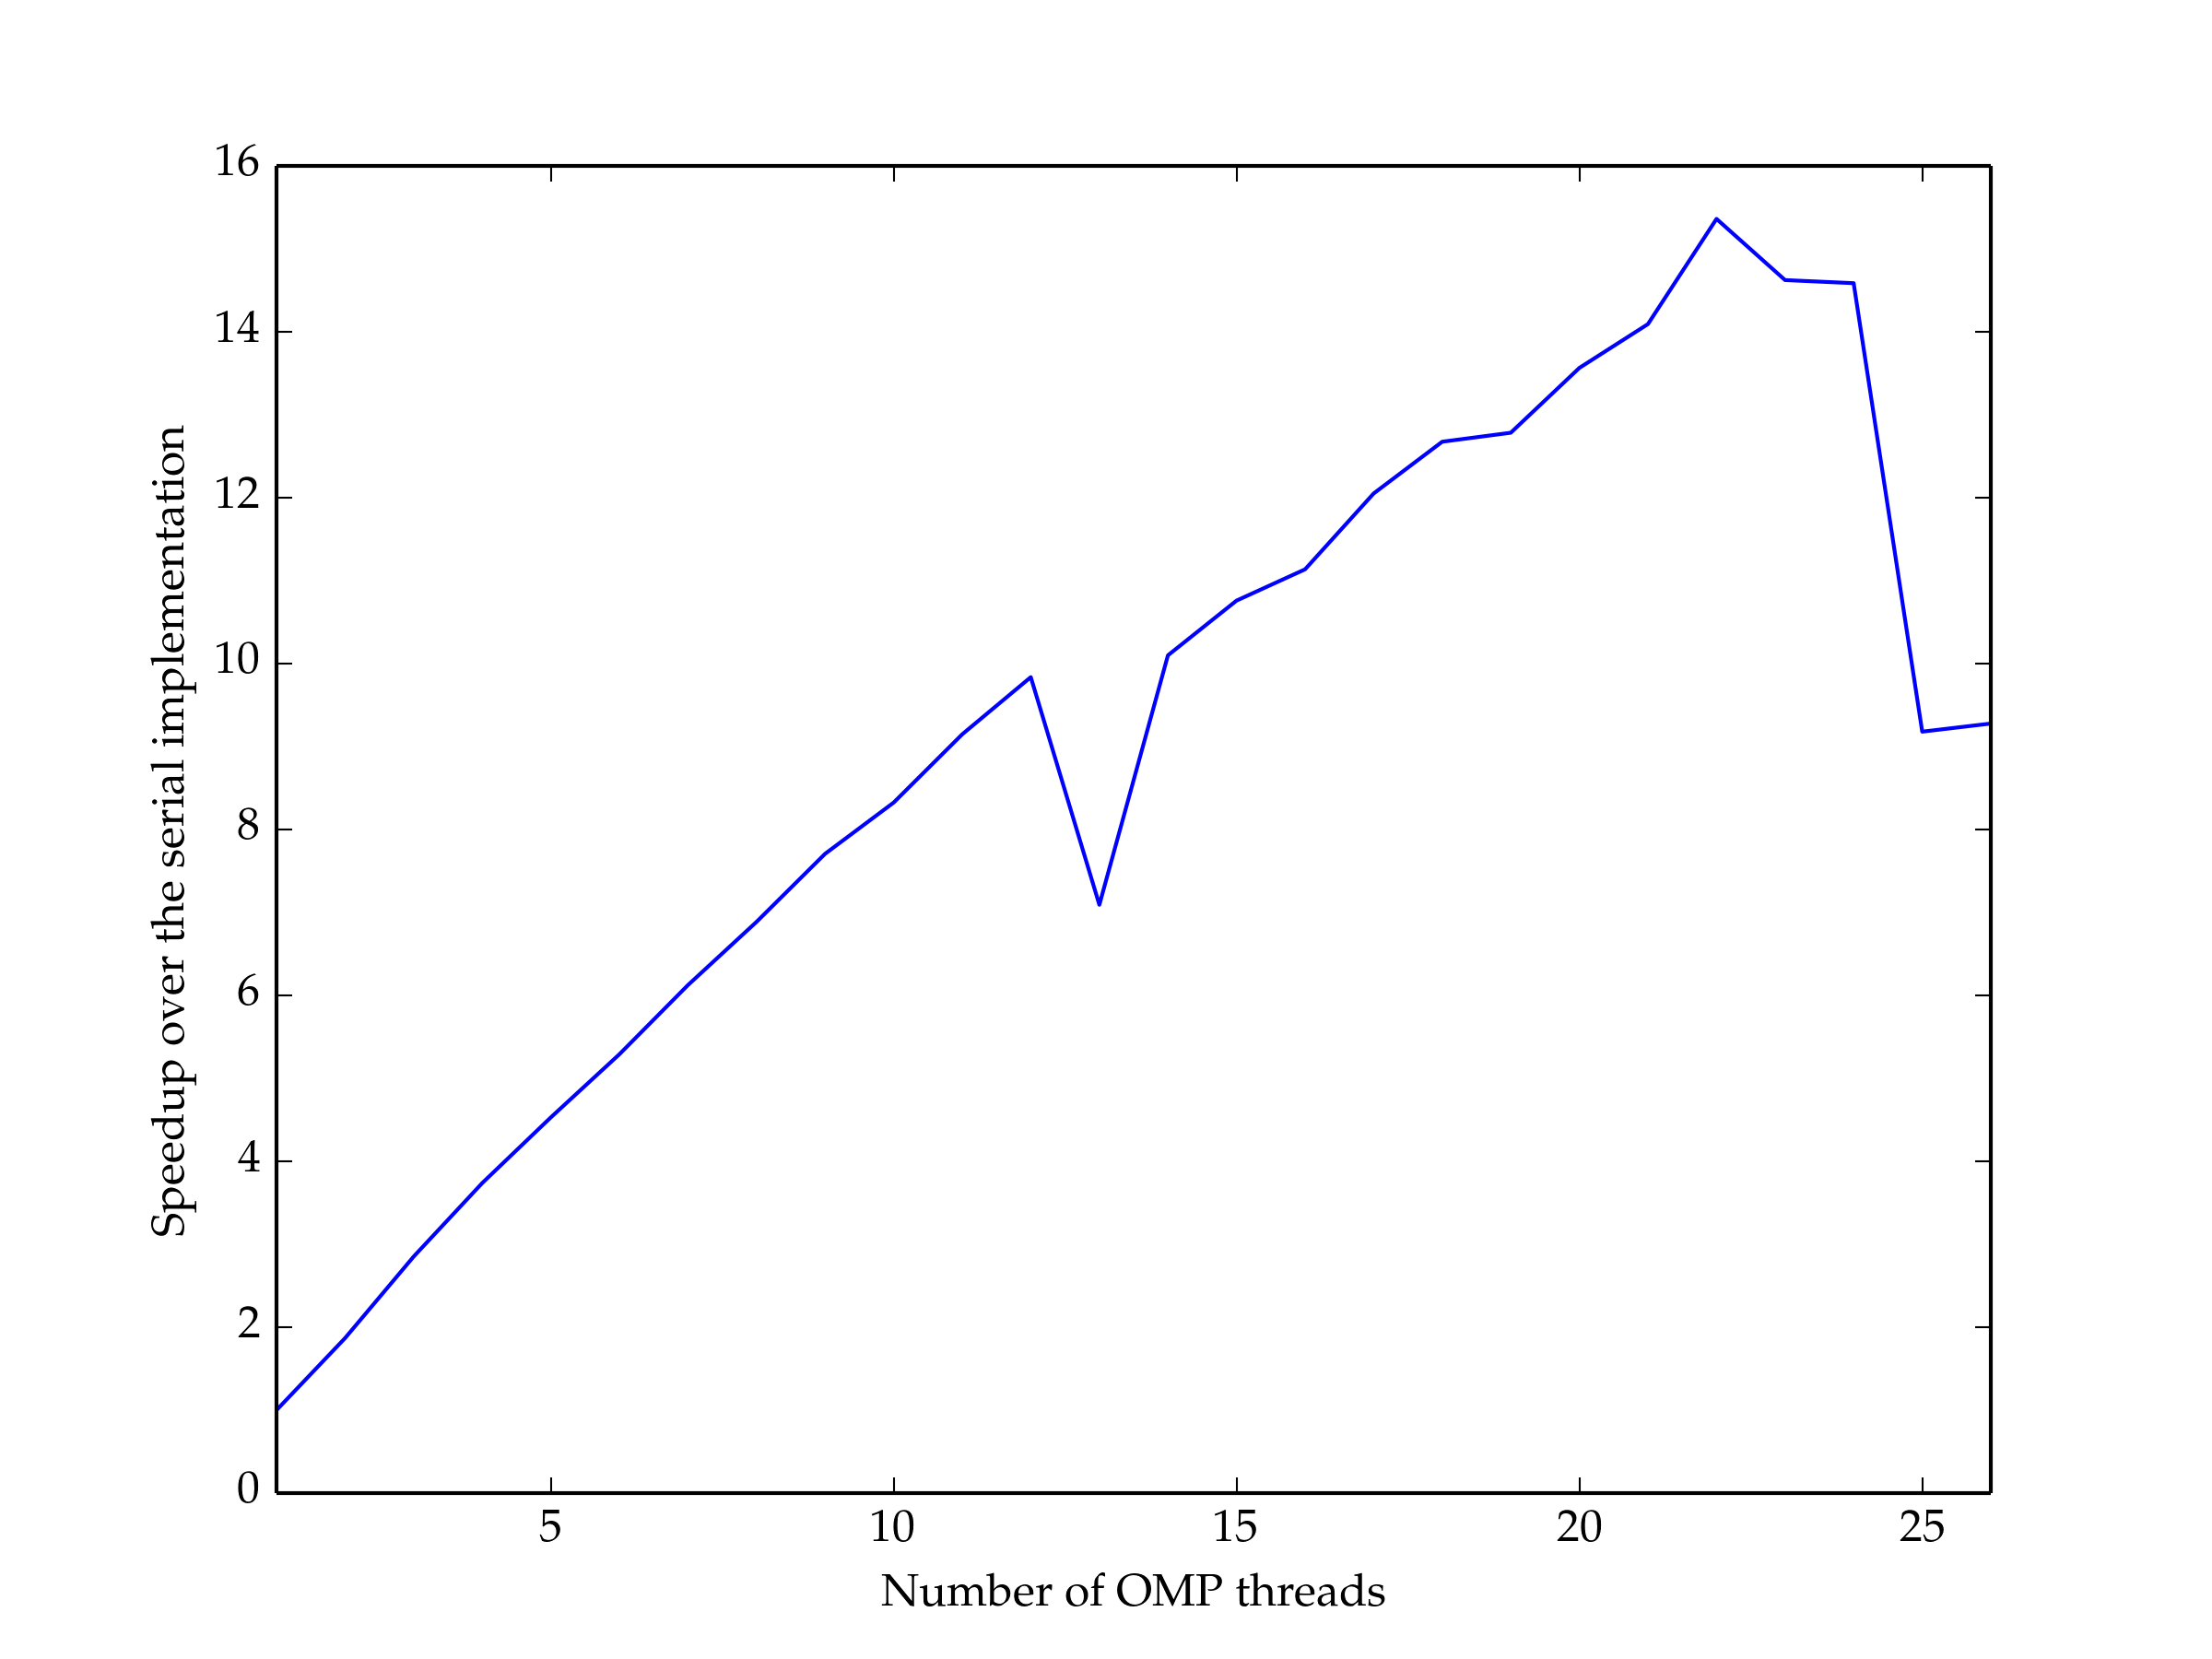
\includegraphics[scale=0.8]{./scaling_studies/strong_scaling_original.png}
\caption{Strong scaling study of the original solution}
\label{fig:ss_orig}
\end{figure}
\subsubsection{Weak Scaling Study}
\begin{figure}[H]
\centering
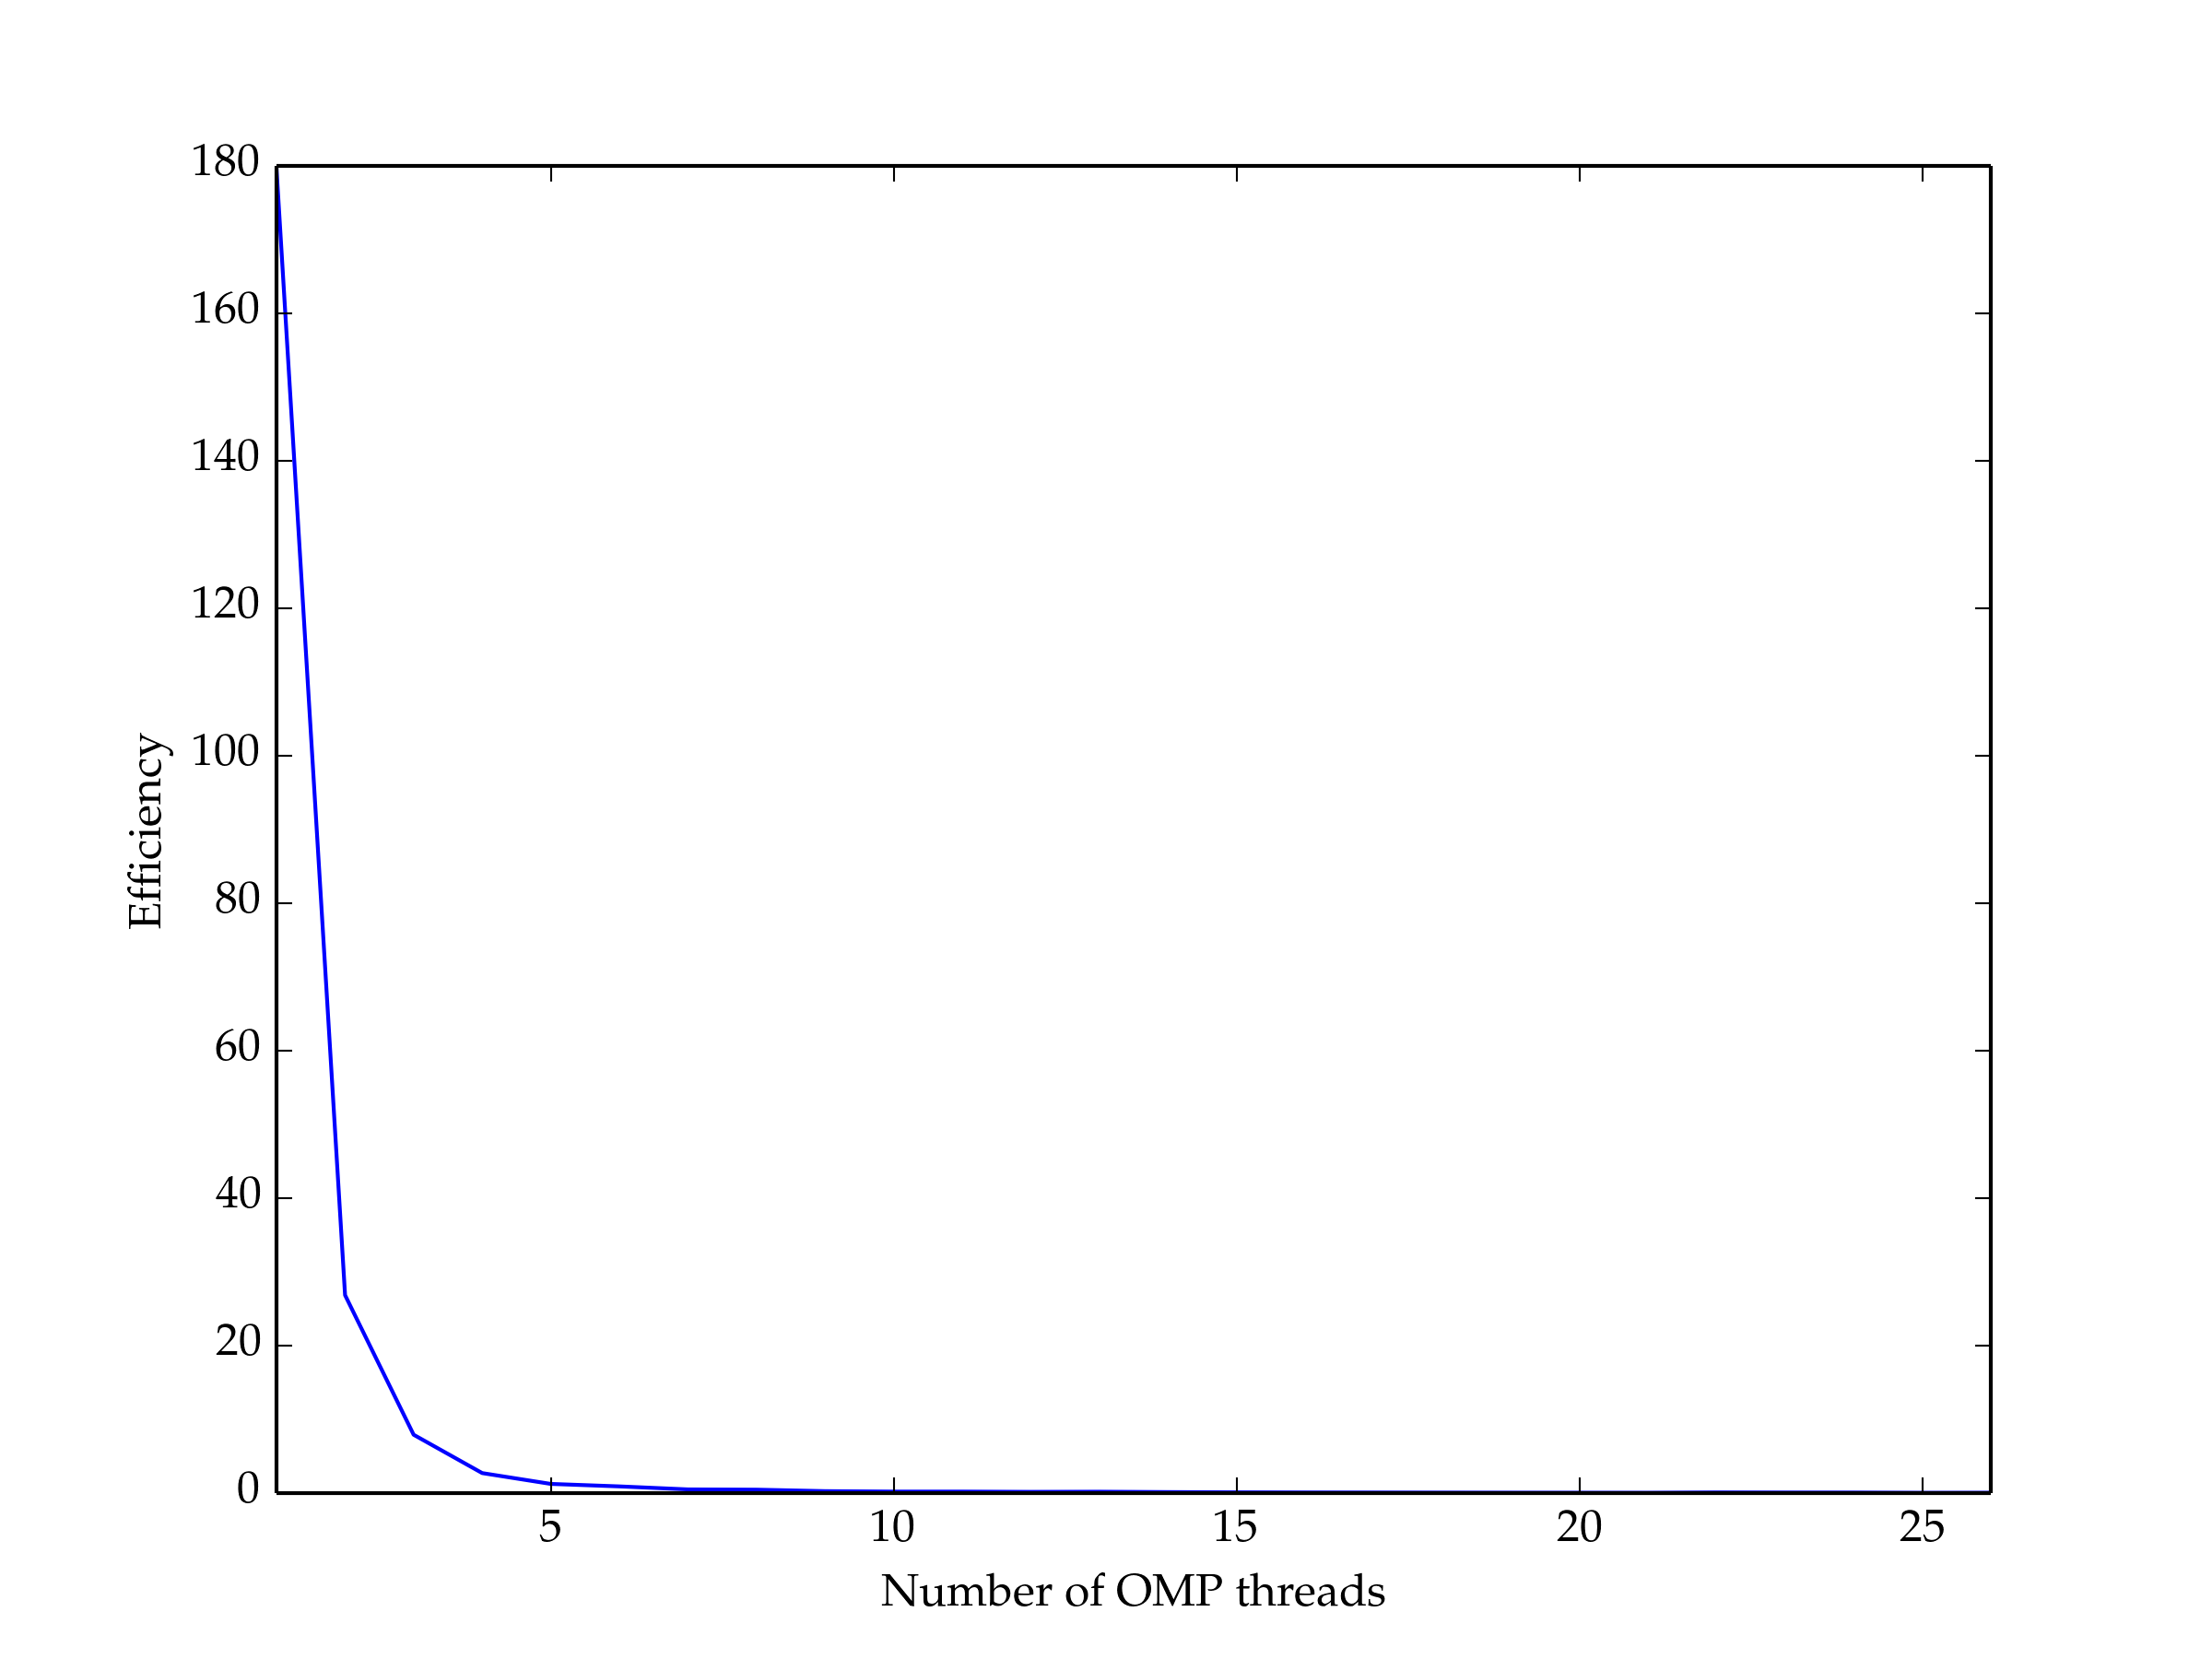
\includegraphics[scale=0.8]{./scaling_studies/weak_scaling_original.png}
\caption{Weak scaling study of the original solution}
\label{fig:ss_orig}
\end{figure}

\subsection{Tuned Parallel Implementation}
\subsubsection{Profiling} \label{sec:prof}
\subsubsection{Scaling Study} \label{sec:speedup}
\subsubsection{Strong Scaling Study}
\subsubsection{Weak Scaling Study}

\subsection{MPI Implementation}
\subsubsection{Profiling} \label{sec:prof}
\subsubsection{Scaling Study} \label{sec:speedup}
\subsubsection{Strong Scaling Study}
\subsubsection{Weak Scaling Study}


\begin{thebibliography}{9}
\bibitem{writeup}
Bindel, D. All-Pairs Shortest Paths. Retrieved November 10, 2015, from \url{https://github.com/sheroze1123/path/blob/master/main.pdf}

\end{thebibliography}

 
 
\end{document}
